\documentclass{article}

\textwidth=6.5in
\textheight=8.5in
\voffset=-54pt
\oddsidemargin=0in
\evensidemargin=0in
\setlength{\parskip}{8pt}
\setlength{\parindent}{0pt}

\usepackage{amsmath, amssymb}
\usepackage{ifthen}

\usepackage[inline]{enumitem}
\setlist{topsep=0pt, parsep=8pt}

\usepackage[rgb,table]{xcolor}\convertcolorsUfalse
\usepackage{graphicx}

% change hyperref options
\PassOptionsToPackage{hyphens}{url}
\usepackage[bookmarks,colorlinks,linkcolor=black,citecolor=blue,pdfstartview=FitH,urlcolor=blue]{hyperref}
\hypersetup{pdfpagemode=UseNone}
\usepackage{bookmark}

\usepackage{graphicx}
\usepackage{multicol}
\usepackage{framed}
\usepackage{array}

\usepackage{icomma}

\usepackage{soul}

\usepackage{pgfplots}
\pgfplotsset{compat=1.18}  
\pgfplotscreateplotcyclelist{mycolor}{black, blue, red, green!70!black, magenta, purple, cyan, orange }  
\pgfplotsset{
  disabledatascaling,
  cycle list=tikzcolor, 
  axis lines=middle,
  every axis plot/.style={no marks, thick},
  every axis/.style={
    enlarge x limits=false,
    enlarge y limits=auto,
    xlabel style={at={(current axis.right of origin)},anchor=west},
    ylabel style={at={(current axis.above origin)},anchor=south},
    % extra x and y ticks for asymptotes
    extra x tick style={grid=major, grid style={dashed,black}},
    extra y tick style={grid=major, grid style={dashed,black}},
    /pgf/number format/1000 sep={},
  },    
  tick label style = {font=\footnotesize, fill=\currentbgcolor, inner sep=0pt},    
  xticklabel shift=1pt,    
  scaled ticks=false,
  scaled y ticks=false,
  unbounded coords=jump,
  samples=101,
  minor tick length=0,
  scatter/classes={
    open={mark=*,draw=black,fill=white, mark size=2, thin},
    closed={mark=*,draw=black,fill=black, mark size=2, thin}
  },
  width=3in,
}
\pgfplotsset{open/.style={only marks, mark=*, fill=white, thin, mark size=2}}
\pgfplotsset{closed/.style={only marks, mark=*, draw=black, fill=black,
    thin, mark size=2}}
\pgfplotsset{labeled/.style={nodes near coords, only marks, mark=*, draw=black, fill=black, thin, mark size=2, point meta=explicit symbolic}}

\usepackage{tikz}
\usetikzlibrary{
  matrix,%
  % enables the snake paths
  decorations.pathmorphing,%
  % enables bigger arrows
  decorations.markings,%
  decorations.pathreplacing,%
  decorations.text,%
  calc,%
  patterns,%
  shapes.geometric,%
  arrows,
  decorations.shapes,
  positioning,
  plotmarks,
  intersections
}
\tikzset{>=latex} % sets default arrow type in tikz
\tikzset{font=\normalsize}
\tikzset{mark size=1.5pt, mark options=thin}
\tikzset{pin distance=4pt,
  every pin edge/.style={<-, thin, shorten <= -2pt}}

\interfootnotelinepenalty=10000
\renewcommand{\thefootnote}{(\arabic{footnote})}

\usepackage{multirow, bigdelim}

% change to \usepackage[sols]{handout} to see solutions
\usepackage[]{handout}

\newcommand\iscurrentenumi[1]{%
  \ifthenelse{\equal{#1}{\theenumi}}{}{#1}}
\setenumerate[1]{ref=\#\arabic*}
\setenumerate[2]{ref=\protect\iscurrentenumi{\theenumi}(\alph*)}
\newcommand\enumiiprefix[2]{%
  \ifthenelse{{\equal{#1}{\theenumi}}\AND{\equal{#2}{(\alph{enumii})}}}{}{}%
  \ifthenelse{{\equal{#1}{\theenumi}}\AND{\NOT{\equal{#2}{(\alph{enumii})}}}}{#2}{}%
  \ifthenelse{\equal{#1}{\theenumi}}{}{#1#2}%
}
\setenumerate[3]{ref=\protect\enumiiprefix{\theenumi}{(\alph{enumii})}\roman*}

\definecolor{purple}{rgb}{0.5,0,1.0}

\newcommand{\doedfinity}[2][\newpage]{
  \begin{problem}[#1]
    Do the Edfinity assignment ``Problem Set #2''.

    We encourage you to write down any scratch work here, as well as
    things you want your future self to remember. Nothing you write
    here will be graded; it's just for you!
  \end{problem}
}

\newcommand{\psrnewpage}{\newpage}
\newcommand{\psreflection}[2][]{

  \ifthenelse{\not\equal{#1}{nocite}}{
    \begin{enumerate}[resume]
    \item
      \begin{problem}[1in]
        Please cite any help you got on this problem set:
        \begin{itemize}[nosep]
        \item If you worked with other students, please list their names here.
        \item If you used resources other than those on our Canvas site, please list them here.
        \end{itemize}
      \end{problem}

    \end{enumerate}
  }

  \probonly{%
    #2

    \psrnewpage

    \emph{Reflection space.} It's a good habit to take a few minutes at the end of each pset to reflect on what you learned and jot down notes to your future self. Here are a few reflection questions to get you started. Nothing you write here will be graded; it's just for you!
    \begin{itemize}
    \item Take a few minutes to look back at the problems. How could you explain to someone else how to do each problem? What was your strategy, and how did you know to use that strategy? If there are problems where you don't feel able to answer this, write down which ones they are. Come back to them in a few days when we post the homework solutions!

      \vspace{1.5in}

    \item Take a look back at the learning objectives on today's worksheet; how are you feeling about each one? If there are ones you know you need more practice with, write those down here.

      \vspace{1.5in}

    \item What did you find most challenging about this material? Do you have any lingering questions about it? If so, write them down here so you don't forget them. At some point, stop by office hours or MQC to ask!

      \vfill
    \end{itemize}      
  }
}

\usepackage{fancyhdr}
\lhead{\textcolor{white}{This content is protected and may not be shared, uploaded, or distributed.}}
\rhead{}
\rfoot{\vspace*{\fill}\footnotesize\textcopyright{} \emph{Harvard Math Ma}}
\renewcommand{\headrulewidth}{0pt}
\pagestyle{fancy}
\begin{document}

\begin{center}
  \large\textsc{Problem Set 14 - More on Limits}\vspace{.5in}\\
  \begin{problemonly}
   \large Name: \rule{5cm}{0.15mm}\\
   \end{problemonly}
\end{center}

\begin{enumerate}
\item  \note{
    \begin{itemize}[nosep]
    \item Practice evaluating limits like those we did last class
    \item Decide whether several statements about combining limits (like: ``If $\displaystyle\lim_{x\to a} f(x) = 0$ and $\displaystyle\lim_{x\to a} g(x) = 0$, then $\displaystyle\lim_{x\to a} \frac{f(x)}{g(x)} = 1$.'') are true.
    \end{itemize}
}

  \doedfinity{14}

\item \label{limits-choose-graph-1}

  \begin{enumerate}
  \item \label{limits-choose-graph-1-evaluate}

    Evaluate the following limits, showing your work and explaining your reasoning very clearly.

    \begin{grading}
      1.5 points per part: 0.5 for the answer, 1 for supporting work\\
      For limits to infinity, if reasoning about dominant terms and similarity in behavior are not clearly shown, deduct between -0.5 and -1, depending on how unclear the reasoning is.
    \end{grading}

    \begin{enumerate} 
    \item
      \begin{problem}[\vfill]
        $\displaystyle \lim_{x \to \infty} \frac{x^2 + 1}{x^3 - 1}$
      \end{problem}

      \begin{solution}
        As we've seen, when taking the limit as $x \to \infty$ of a sum, we need to identify the fastest growing term (the highest power of $x$). 
        \begin{itemize}
            \item In the numerator, as $x \to \infty$ we find $x^2>>1$, so $x^2+1 \sim x^2$.
            \item In the denominator, as $x \to \infty$, we find $x^3>>-1$, so $x^3-1 \sim x^3$.
        \end{itemize}
        Taking this into account, we can reason the following:
        \[
          \lim_{x \to \infty} \frac{x^2 + 1}{x^3 - 1} = \lim_{x \to \infty} \frac{x^2}{x^3}
          = \lim_{x \to \infty} \frac{1}{x} = 0.
        \]
      \end{solution}

    \item
      \begin{problem}[\vfill]
        $\displaystyle \lim_{x \to -\infty} \frac{x^2 + 1}{x^3 - 1}$
      \end{problem}

      \begin{solution}
      Here are our observations about the parts of this function:
        \begin{itemize}
            \item In the numerator, as $x \to -\infty$ we find $x^2>>1$, so $x^2+1 \sim x^2$.
            \item In the denominator, as $x \to -\infty$, we find $x^3>>-1$, so $x^3-1 \sim x^3$.
        \end{itemize}
        \[
          \lim_{x \to -\infty} \frac{x^2 + 1}{x^3 - 1} = \lim_{x \to -\infty} \frac{x^2}{x^3}
          = \lim_{x \to -\infty} \frac{1}{x} = 0.
        \]
      \end{solution}

    \item
      \begin{problem}[\vfill]
        $\displaystyle \lim_{x \to 1^-} \frac{x^2 + 1}{x^3 - 1}$
      \end{problem}

      \begin{solution}
        Direct substitution gives $\frac{2}{0}$, which is undefined, but we now need to determine whether the denominator is approaching zero from the positive or the negative side, which will help us determine the limit. As $x$ approaches $1$ from the left, the numerator is positive
        and the denominator is negative, so
        \[\lim_{x \to 1^-} \frac{x^2 + 1}{x^3 - 1}=-\infty.\]
      \end{solution}

    \item
      \begin{problem}[\vfill]
        $\displaystyle \lim_{x \to 1^+} \frac{x^2 + 1}{x^3 - 1}$
      \end{problem}

      \begin{solution}
        Direct substitution gives $\frac{2}{0}$. We more closely investigate the direction of approach as we did in the previous part. As $x$ approaches $1$ from the right, the numerator is positive
        and the denominator is positive, so
        \[\lim_{x \to 1^-} \frac{x^2 + 1}{x^3 - 1}=\infty.\]
      \end{solution}

    \end{enumerate} 

  \item

    \begin{grading}
      1 point
    \end{grading}

    \begin{problem}
      One of the following pictures is the graph of $\displaystyle \frac{x^2 + 1}{x^3 - 1}$. Which one? (How does \ref{limits-choose-graph-1-evaluate} help you answer this question?) No explanation is necessary.
    \end{problem}

    {%
      \pgfplotsset{%
        every axis/.append style={domain=-5:5, xtick=\empty, ytick=\empty,
          extra x ticks={1}, width=1.75in, height=1.75in, ymin=-5,
          ymax=5}%
      }

      \begin{tabular}{c c c c}
        \begin{tikzpicture}
          \begin{axis}
            \addplot+ {(x^2+1)/(x^3-1)};
          \end{axis}
        \end{tikzpicture} &
        \begin{tikzpicture}
          \begin{axis}
            \addplot+[domain=-5:0.99]{(1-x^4/3)/(x^3-1)};
            \addplot+[domain=1.01:5]{(1-x^4/3)/(x^3-1)};
          \end{axis}
        \end{tikzpicture} &
        \begin{tikzpicture}
          \begin{axis}
            \addplot+ {(x^2+1)/abs(x^3-1)};
          \end{axis}
        \end{tikzpicture} &
        \begin{tikzpicture}
          \begin{axis}
            \addplot+{(x^4+1)/(x^3-1)};
          \end{axis}
        \end{tikzpicture} \\
        (A) & (B) & (C) & (D)
      \end{tabular}
    }

    \pspace{\nstretch{0.25}}

    \begin{solution}
      The only choice that matches the limits we found in
      \ref{limits-choose-graph-1-evaluate} is \fbox{(A)}.
    \end{solution}

  \end{enumerate}

\item  \begin{enumerate}
  \item

    Evaluate the following limits algebraically. If a limit does not exist, evaluate both one-sided limits. Show your work / explain your reasoning.

    \begin{grading}
      1.5 points each: 0.5 for the answer, 1 for work / explanation\\
      For limits to infinity, if reasoning about dominant terms and similarity in behavior are not clearly shown, deduct between -0.5 and -1, depending on how unclear the reasoning is.
    \end{grading}      

    \begin{enumerate}

    \item

      \begin{problem}[\vfill]
        $\displaystyle \lim_{x \rightarrow -\infty} \frac{x^2 - 3x - 4}{2x - 8}$
      \end{problem}

      \begin{solution}
      We collect our observations about the numerator and denominator separately first:
      \begin{itemize}
          \item In the numerator, we see that as $x \to -\infty$, $x^2>>-3x>>-4$, so $x^2-3x-4 \sim x^2$.
          \item In the numerator, we see that as $x\to -\infty$, $2x>>-8$, so $2x-8 \sim 2x$
      \end{itemize}
        \begin{align*}
          \lim_{x \to -\infty} \frac{x^2 - 3x - 4}{2x - 8} &= \lim_{x \to -\infty} \frac{x^2}{2x} \\
          &= \lim_{x \to -\infty} \frac{x}{2} \\
          &= -\infty
        \end{align*}
      \end{solution}

    \item

      \begin{problem}[\vfill]
        $\displaystyle \lim_{x \rightarrow -1} \frac{x^2 - 3x - 4}{2x - 8}$
      \end{problem}

      \begin{solution}
        \begin{align*}
          \lim_{x \to -1} \frac{x^2 - 3x - 4}{2x - 8} &= \frac{(-1)^2 - 3(-1) - 4}{2(-1)-8}\\
          &= \frac{0}{-10} \\
          &= 0.
        \end{align*}
      \end{solution}

    \item

      \begin{problem}[\vfill]
        $\displaystyle \lim_{x \rightarrow 4} \frac{x^2 - 3x - 4}{2x - 8}$
      \end{problem}

      \begin{solution}
        \begin{align*}
            \lim_{x \to 4} \frac{x^2 - 3x - 4}{2x - 8} 
            &= \lim_{x \to 4} \frac{(x-4)(x+1)}{2(x-4)} \\
          &= \lim_{x \to 4} \frac{x+1}{2} \\
          &= \frac{5}{2}.
        \end{align*}
      \end{solution}
    \end{enumerate}

  \item

    \begin{grading}
      3 points: 1 for the graph looking like $\dfrac{x + 1}{2}$, 1 for having a hole at $x = 4$, 1 for explanation
    \end{grading}

    \begin{problem}[\nstretch{2}]
      Graph $f(x) = \displaystyle \frac{x^2 - 3x - 4}{2x - 8}$, explaining how you got the graph. (You should be able to do this by hand!) Make sure your answers to the previous parts are consistent with your graph.
    \end{problem}

    \begin{solution}
      Since $f(x) = \dfrac{x^2 - 3x - 4}{2x - 8} = \dfrac{(x-4)(x+1)}{2(x-4)}=\frac{1}{2}(x+1), x\neq 4$, the graph is just the graph
       of $y=\frac{1}{2}x + \frac{1}{2}$, but with a hole at $x=4$.
       
       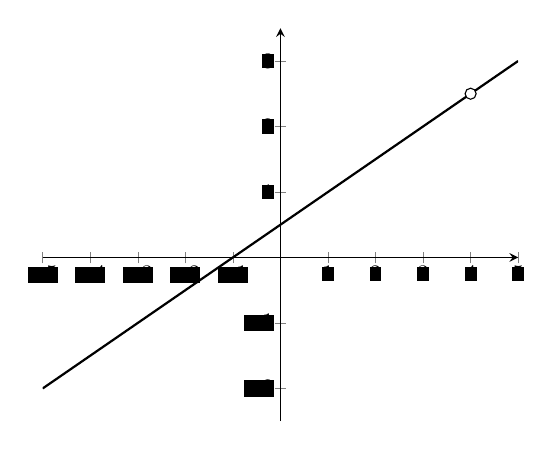
\begin{tikzpicture}
          \begin{axis}[xtick distance=1, ytick distance=1]
            \addplot[domain=-5:5] {0.5*x+0.5};
            \addplot[open] coordinates {(4, 2.5)};
          \end{axis}
       \end{tikzpicture}
    \end{solution}

  \end{enumerate}

\item \label{graphical-limit-2-functions-1} 

  The graphs of $f$ and $g$ are given below.

  \begin{center}
    \begin{tikzpicture}
      \begin{axis}[xmin=-3.5, xmax=3.5, axis equal=true, xtick={-3, -2, ..., 3}]
        \addplot+[domain=-3:-1] {x+2};%
        \addplot+[domain=-1:1] {2};%
        \addplot+[domain=1:2] {(x-1)^2};%
        \addplot+[domain=2:3] {-1};%
        \addplot[closed] coordinates { (-3, -1) (-1, 1) (2, -1) (3, -1) (1, 2) };%
        \addplot[open] coordinates { (-1, 2) (1, 0) (2, 1) };%
        \draw (axis cs: 3, 3) node{$f$};%
      \end{axis}
    \end{tikzpicture}
    \hspace{0.5in}
    \begin{tikzpicture}
      \begin{axis}[xmin=-3.5, xmax=3.5, axis equal=true, xtick={-3, -2, ..., 3}]
        \addplot+[domain=-3:-1] {1};%
        \addplot+[domain=-1:1] {-x};%
        \addplot+[domain=1:3] {abs(x-2)};%
        \addplot[closed] coordinates { (-3, 1) (-1, 2) (3, 1) (1, -1) };%
        \addplot[open] coordinates { (-1, 1) (1, 1) };%
        \draw (axis cs: 3, 3) node{$g$};%
      \end{axis}
    \end{tikzpicture}    
  \end{center}  

  Evaluate each limit, and explain your reasoning briefly.

  \begin{enumerate}
  \item

    \begin{grading}
      1 point
    \end{grading}

    \begin{problem}[\vfill]
      $\displaystyle \lim_{x \to 0} [f(x) + g(x)]$
    \end{problem}

    \begin{solution}
      We have $\displaystyle\lim_{x \to 0} f(x) = 2$ and $\displaystyle\lim_{x \to 0} g(x) = 0$, so the sum of these two functions is approaching $\boxed{2}$ as $x$ gets close to $0$. 
    \end{solution}

  \item

    \begin{grading}
      This part and the remaining parts are 2 points each: 0.5 for recognizing they need to look at one-sided limits, 0.5 for reasoning about each one-sided limit, 0.5 for the conclusion.
    \end{grading}

    \begin{problem}[\vfill]
      $\displaystyle \lim_{x \to 1} [f(x) + g(x)]$
    \end{problem}

    \begin{solution}
      $f$ and $g$ are not so well-behaved at 1, but they are on either side of 1, so we can evaluate each one-sided limit. We have 
      \begin{align*}
        \lim_{x \to 1^-} \big[ f(x) + g(x) \big] &= 2 + (-1) \\
        \lim_{x \to 1^+} \big[ f(x) + g(x) \big] &= 0 + 1
      \end{align*} 
      and both one-sided limits equal $1$. So the original limit is also $\boxed{1}$.
    \end{solution}

  \item
    \begin{problem}[\vfill]
      $\displaystyle \lim_{x \to 1} f(x) g(x)$
    \end{problem}

    \begin{solution}
      We again compute left and right handed limits 
      \begin{align*} 
        \lim_{x \rightarrow 1^+} f(x) g(x) &= 0 \cdot 1\\
        \lim_{x \rightarrow 1^-} f(x) g(x) &= 2 \cdot (-1) 
      \end{align*} 
      Since the left hand limit does not equal the right hand limit, the limit does not exist. 
    \end{solution}

  \item
    \begin{problem}[\vfill\newpage]
      $\displaystyle \lim_{x \to 1} [g(x)]^2$
    \end{problem}

    \begin{solution}
      We'll evaluate each one-sided limit as usual:  
      \begin{align*}
        \lim_{x \to 1^-} \Big[ g(x) \Big]^2 &= (-1)^2 \\
        \lim_{x \to 1^+} \Big[ g(x) \Big]^2 &= 1^2
      \end{align*}  
      and both these one-sided limits are equal, to $\boxed{1}$.
    \end{solution}

  \end{enumerate}

\item  \label{limits-sketch-discontinuities}

  In each part, sketch a function $f(x)$ with the specified properties.

  \begin{grading} 
    2 points each.
  \end{grading} 

  \begin{enumerate}
  \item
    \begin{problem}[\vfill]
      $\displaystyle \lim_{x \to 3} f(x)$ exists, but $f(3)$ does not.
    \end{problem}

    \begin{solution}
      \begin{center}
        \begin{tikzpicture}
          \begin{axis}[xtick={3}]
            \addplot+[domain=0:5] {(x - 1) * (x - 2) * (x - 4)};%
            \addplot[open] coordinates { (3, -2) };%
          \end{axis}
        \end{tikzpicture}
      \end{center}
    \end{solution}

  \item 
    \begin{problem}[\vfill]
      $\displaystyle \lim_{x \to 3} f(x)$ and $f(3)$ both exist, but they are not equal to each other.
    \end{problem}

    \begin{solution}
      \begin{center}
        \begin{tikzpicture}
          \begin{axis}[xtick={3}]
            \addplot+[domain=0:5] {(x - 1) * (x - 2) * (x - 4)};%
            \addplot[open] coordinates { (3, -2) };%
            \addplot[closed] coordinates { (3, -7) };%
          \end{axis}
        \end{tikzpicture}
      \end{center}
    \end{solution}

  \item 
    \begin{problem}[\vfill\newpage]
      $\displaystyle \lim_{x \to 3} f(x)$ and $f(3)$ both exist, and they are  equal to each other.
    \end{problem}

        \begin{solution}
      \begin{center}
        \begin{tikzpicture}
          \begin{axis}[xtick={3}]
            \addplot+[domain=0:5] {(x - 1) * (x - 2) * (x - 4)};%
          \end{axis}
        \end{tikzpicture}
      \end{center}
    \end{solution}

  \item
    \begin{problem}[\vfill]
      $\displaystyle \lim_{x \to 3} f(x)$ does not exist, but $f(3)$
      does.
    \end{problem}

    \begin{solution} 
      \begin{center}
        \begin{tikzpicture}
          \begin{axis}[xtick={3}]
            \addplot+[domain=0:3] {(x - 1) * (x - 2) * (x - 4)};%
            \addplot+[domain=3:5] {(x - 1) * (x - 2) * (x - 4) - 5};%
            \addplot[open] coordinates { (3, -2) };%
            \addplot[closed] coordinates { (3, -7) };%
          \end{axis}
        \end{tikzpicture}
      \end{center}
    \end{solution}

  \item
    \begin{problem}[\vfill]
      Neither $\displaystyle \lim_{x \to 3} f(x)$ nor $f(3)$ exists. 
    \end{problem}

        \begin{solution} 
      \begin{center}
        \begin{tikzpicture}
          \begin{axis}[xtick={3}]
            \addplot+[domain=0:3] {(x - 1) * (x - 2) * (x - 4)};%
            \addplot+[domain=3:5] {(x - 1) * (x - 2) * (x - 4) - 5};%
            \addplot[open] coordinates { (3, -2) (3, -7) };%
          \end{axis}
        \end{tikzpicture}
      \end{center}
    \end{solution}

  \end{enumerate} 

\end{enumerate}
\psreflection{}
\end{document}
